% This is LLNCS.DOC the documentation file of
% the LaTeX2e class from Springer-Verlag
% for Lecture Notes in Computer Science, version 2.4
\documentclass{llncs}
\usepackage{llncsdoc}
\usepackage{graphicx}
\usepackage{amssymb}
\usepackage{amsmath}
\usepackage[table]{xcolor}

\usepackage{url}
\urldef{\mailwhajwp}\path|{homenda,A.Jastrzebska}@mini.pw.edu.pl, waszkiewiczp@student.mini.pw.edu.pl|
\newcommand{\keywords}[1]{\par\addvspace\baselineskip
\noindent\keywordname\enspace\ignorespaces#1}
%
\begin{document}


\title{Regression Models for Classification \\with Foreign Patterns Rejection}
\author{Wladyslaw Homenda$^{1}$
\and Agnieszka Jastrzebska$^1$
\and Piotr Waszkiewicz$^{1}$
}

\authorrunning{W. Homenda, A. Jastrzebska, and P. Waszkiewicz}
\institute{$^1$Faculty of Mathematics and Information Science, Warsaw University of Technology\\ul. Koszykowa 75, 00-662 Warsaw, Poland\\
%$^2$Department of Electrical \& Computer Engineering, University of Alberta, \\Edmonton T6R 2G7 AB Canada\\
\mailwhajwp
}

\titlerunning{Regression Models for Classification with Foreign Patterns Rejection}
\maketitle

\pagestyle{empty}  % no page numbers, no running headers

\begin{abstract}
In the article we discuss the issue of contaminated data sets that which, apart from proper patterns, contain improper elements. To distinguish between those two kinds of patterns we use terms: native (proper patterns) and foreign (garbage patterns). We do not know neither origins, nor characteristics of foreign patterns. They can appear in the data, for example when signal segmentation algorithm is poorly, or when input streams get mixed. Foreign patterns do not belong to any native class, and therefore we do not want to account them as native. Ideally, we wish to remove them from the data entirely. However, due to the mentioned obstacles (unknown characteristics), foreign patterns rejection mechanism  should not be trained based on some synthetic substitute foreign patterns as such course of actions will limit rejection mechanism's capability for generalization to various unexpected foreign patterns. To deal with the issue of contaminated data sets in this paper we propose to build foreign patterns rejection mechanism based on a~collection of regression models. We propose a~scheme for a~classifying/rejecting model for a multi-class data set trained entirely on native patterns. The developed approach is tested in a~study of handwritten digits recognition. 
\end{abstract}


%-------------------------------------------------------------------
%-------------------------------------------------------------------
%-------------------------------------------------------------------

\section{Introduction}
  \label{sec:Introduction}

Pattern recognition is a~classical machine learning problem. Its aim is to form a~model (called classifier) that, after initial training, can assign correct class labels to new patterns. The training process usually consists of feeding example data to classifier and providing answers in form of proper labels for each pattern in a~training set. The ideal situation occurs when trained model is properly classifying patterns from outside of the training dataset, which means it gained ability to generalise information. 

It is important to have in mind that patterns in their original form are usually some sort of a~signal, for instance images or voice recordings. Due to the fact, that original patterns are often collected automatically with some signal-acquiring device, patterns that should not be accounted to any of proper classes may be recorded. Such situation may happen, when a~device that is used to acquire data was automatically reset due to a~power outage and a~poor default calibration hinders signal segmentation process. Another scenario is when we collect data in a~noisy (out of lab) environment and, apart from proper patterns, there is a~lot of unexpected and unwanted input. The main problem with such erroneous patterns, called foreign patterns, is that their characteristics cannot be easily predicted and therefore cannot be included in the model training process.

The motivation for our study is to provide algorithmic approaches used for distinguishing proper patterns (called \emph{native patterns}) from garbage and unwanted ones (called \emph{foreign patterns}) by using only classifiers for both rejection and classification. The design assumption is to provide methods based on native patterns only so that the approach could be truly versatile and could be easily adapted to any pattern recognition problem in an uncertain environment, where foreign patterns may appear. The study focuses on a~multi-class pattern recognition problem, for which we employ specifically constructed classification models that together perform actions of classification and rejection. It should be emphasised that novelty of the contribution presented in this paper is in the application of otherwise well-known methods to a~new area of study. 

The remainder of this paper is organized as follows. Section~\ref{sec:Literature Review} presents the background knowledge on foreign patterns detection present in the literature. Section~\ref{sec:Known algorithms} presents the backbone algorithms, known in the literature, that were used to construct our models. Section~\ref{sec:rejectionmechanism} presents the proposed approach. Section~\ref{sec:Experiments} discusses a~series of experiments. Section~\ref{sec:Conclusion} concludes the paper and highlights future research directions.
\vspace{-3pt}

%-------------------------------------------------------------------
%-------------------------------------------------------------------
%-------------------------------------------------------------------
\section{Literature Review}
  \label{sec:Literature Review}
The problem of contaminated data sets has been reappearing in research on pattern recognition in various contexts. First studies, which we may account as tightly related to foreign patterns rejection, were dealing with outliers detection. Outliers are proper native patterns, whose characteristics significantly differ from the majority of data. Outliers, due to their atypical character, may cause problems at a~model training stage. Therefore, we are often advised to apply a~variety of methods to detect them and, if needed, to modify or remove from the set of native patterns before further processing. Literature provides us with a~selection of statistical tests, for instance discussed in~\cite{Grubbs1950,Tukey1977}, which act as decision rules for outlier detection. Apart from statistical tests, we find more convoluted approaches. In particular, there is a~wide variety of methods related to the notion of distance. Those methods evaluate either proximity of data points or their density in order to detect outliers. Popular examples of such approaches have been presented in~\cite{BreunigKriegelNgSander1999,KnorrNg1999}.

We shall stress that foreign patterns are not outliers. When it comes to outliers, we can actually determine their proper class belongingness, even though it is difficult. In contrast, foreign patterns do not belong to any class and should be removed from the data. 

An area of studies, which is even more similar to foreign patterns rejection, is the so called novelty detection. Novelty elements are patterns that belong to extremely infrequent native classes. A~typical domain, in which we recognize the importance of novelty elements, is text processing. Even large corpora of texts often contain meaningful, but rare key phrases. Studies on novelty detection typically utilize either a~probabilistic approach or are based on the notion of distance,~\cite{PimentelCliftonTarassenko2014}. Among successful probabilistic approaches we can find kernel density estimators, as for example reported in~\cite{Kapoor2010,KimLee2006}, and mixture models (for instance discussed in~\cite{Paalanen2006,Song2007}). The goal of these methods is to perform probability density estimation of the data. In contrast, distance-based methods for novelty detection rely on the assumption that novel elements are located far from majority of data. In this line of study, we find methods resolving to various sophisticated distance measures, for instance~\cite{Chawla2006,Ghoting2008} or even methods based on well-known clustering algorithms, as for example in~\cite{He2003,Sun2004}.

Foreign elements detection, alike novelty detection task, has to assume that native patterns, alike majority class, is the only available information. Therefore, model construction has to rely on native patterns only. In this paper we present a~method for foreign patterns rejection based on classifying models. The approach that we work on is fit to solve multi-class classification problems (when more than two native classes are present). The proposed technique uses a~collection of specifically trained binary classifiers, which set together to form a~specific structure provide capability not only to classify native patterns, but also to reject foreign patterns. 
\vspace{-3pt}

%-------------------------------------------------------------------
%-------------------------------------------------------------------
%-------------------------------------------------------------------
\section{Preliminaries}
  \label{sec:preliminaries}

The issue of contaminated data sets frequently emerges from a~substantial automation of data acquisition and processing, that results in poor data quality. The research that we present in this paper has been motivated by the need for algorithmically-aided methods for data sets purging: accepting proper patterns and rejecting foreign. We deal with possibly contaminated multi-class data sets (this is the input). As an output we wish to obtain a~classified data set of native patterns, without foreign elements. In the study addressed in this paper we concentrated on enhancing well-known classifiers in order to perform a~rejection task. We focused on regression models, but we also applied other popular classification algorithms, such as Support Vector Machines (SVM), random forest and k-Nearest Neighbours (kNN). In what follows we discuss applied algorithms. First, we address well-known classification models applied in the study. Second, in Section~\ref{sec:rejectionmechanism} we discuss our approach to rejection mechanism construction, based on those algorithms. Finally, we address quality measures.
\vspace{-3pt}

%-------------------------------------------------------------------
%-------------------------------------------------------------------
\subsection{The Task of Classification with Rejection}
	\label{sec:Known algorithms}

The task of classification aims at categorising unknown elements to their appropriate groups. The procedure is based on quantifiable characteristics obtained from the source signal. Those characteristics, i.e.~features, are gathered in a~feature vector (a~vector of independent variables) and each pattern is described with one feature vector. We expect that patterns accounted to the same category are in a~relationship with one another. In other words, subjects and objects of knowledge accounted to the same category are expected to be in some sense similar. There are many mathematical models that can be used as classifiers, such as SVM, random forest, kNN, regression models, or Neural Networks. Their main disadvantage lies in their need to be trained prior to usage, which makes them unable to recognize elements from a~new class, not present during the training process. This behaviour can be especially troublesome in an unstable, noisy environment, where patterns sent for classification can be corrupted, distorted or otherwise indistinguishable. In such situation a~proper mechanism for rejecting garbage patterns could be used to provide correct results. 
\vspace{-3pt}

%-------------------------------------------------------------------
%-------------------------------------------------------------------
\subsection{Support Vector Machines}

Support Vector Machines (SVM) are a~collection of supervised learning methods used for classification, regression and outliers detection. The SVM algorithm relies on a~construction of hyperplane with a~maximal margin that separates patterns of two classes,~\cite{CortesVapnik1995}. SVMs are effective in high-dimensional spaces, memory efficient, and quite versatile with many kernel functions that can be specified for the decision function. Although in some cases, where the number of features is much greater than the number of samples, this method can give poor results, and is not cost-efficient when calculating probability estimates.
\vspace{-3pt}

%-------------------------------------------------------------------
%-------------------------------------------------------------------
\subsection{Random Forest}

Random forest is a~popular ensemble method. The main principle behind ensemble methods, in general, is that a~group of ``weak learners'' can come together to form a~``strong learner''. In the random forest algorithm~\cite{Breiman2001} the weak learners are decision trees, which are used to predict class labels. For a~feature vector representing one pattern a~decision tree calculates its class label by dividing value space into two or more subspaces. More precisely, an input data is entered at the top of the tree and as it traverses down the tree the data gets bucketed into smaller and smaller subsets. In the random forest we form a~large number of classification trees, which altogether serve as a~classifier. In order to grow each tree, we draw with replacement a~random selection of rows from the training set. Random sampling with replacement is also called bootstrap sampling. In addition, when constructing trees for a~random forest at each node we select randomly $m$~variables out of the set of all input variables, and the best split on these $m$~is used to split the node. After a~relatively large number of trees is generated, they vote for the most popular class. Random forests join few important benefits: (a)~they are relatively prone to the influence of outliers, (b)~they have an embedded ability of feature selection, (c)~they are prone to missing values, and (d)~they are prone to overfitting. 

%-------------------------------------------------------------------
%-------------------------------------------------------------------
\subsection{k-Nearest Neighbors}

The k-Nearest Neighbours algorithm, denoted as kNN, is an example of a~``lazy classifier'', where the entire training dataset is the model. There is no typical model building phase, hence the name. Class membership is determined based on class labels encountered in $k$~closest observations in the training dataset,~\cite{Altman1992}. In a~typical application, the only choice that the model designer has to make is selection of $k$~and distance metrics. Both are often determined experimentally with a~help of supervised learning procedures.

%-------------------------------------------------------------------
%-------------------------------------------------------------------

\subsection{Regression}
% regression, description of variants used in the experiments
Regression analysis is a~statistical method for describing relationships between variables. It is applied in order to predict future values of a~given dependent variable based on known values of other variables (independent variables). Regression model construction resolves to formation of a~function that describes how expected value of the dependent variable is related with one or more independent variables. When we deal with more than one independent variable, we have the case of multiple regression. The function can literally be a~mathematical formula, but it can also be an algorithm taking us from the space of independent variables values to the space of depended variables values. Examples of algorithms building a~regression model are: regression trees, neural networks, etc.

Typically, we deal with parametric regression models, where the shape of the regression function is known beforehand and our goal is to determine its components (parameters). When we apply the same set of parameters for all input variables, no matter their particular values, we have the case of global parametric regression. A~general formula for parametric regression is given as follows:
  \vspace{-3pt}
\begin{equation} 
\label{eq:regression} 
Y = f(X, \beta) + \epsilon
\end{equation}
where $Y$~is the dependent variable, $X$~is the vector of independent variables, $\beta$~is the vector of regression coefficients, $f$~is  regression function with values in real numbers, $\epsilon$~is random error. The estimation target is a~function of the independent variables $f$. The goal is to find such a~function that minimizes loss. 

There are many different regression models: linear regression, polynomial regression, logistic regression, Bayesian Ridge regression, etc. In this paper we will focus mainly on two regression variants: logistic and polynomial regression (please note that linear regression is in fact polynomial regression using polynomial of degree~$2$). 

\vspace{-3pt}
\paragraph{Linear regression} is the simplest regression model. It describes the relationship between scalar dependent variable and one or more explanatory variables. For example, if we have three independent variables, multiple regression model looks as follows: \vspace{-3pt}
\begin{equation} 
\label{eq:lineraregression} 
Y = \beta_{0} + \beta_{1}x_{1} + \beta_{2}x_{2} + \beta_{3}x_{3} 
\end{equation} 

\paragraph{Polynomial regression} can be viewed as a~model that uses linear regression extended by constructing polynomial features from the coefficients. This approach maintains the generally fast performance of linear methods, while allowing them to fit to a~much wider range of data. The predictors resulting from the polynomial expansion of the ``baseline'' predictors are known as interaction features, and can be used in classification problem. Just like linear regression, polynomial regression models are usually fit using the method of least squares. Polynomial regression does not contain in its formula interactions between predictors. For instance, if we have three independent variables, polynomial regression quadratic model looks as follows:\vspace{-3pt}
\begin{equation} 
\label{eq:polynomialregression} 
Y = \beta_{0} + \beta_{1}x_{1} + \beta_{2}x_{1}^{2} + \beta_{3}x_{2} + \beta_{4}x_{2}^{2}  + \beta_{5}x_{3} + \beta_{6}x_{3}^{2}
\end{equation} 


\paragraph{Logistic regression} is a regression variant applicable to a~case, when dependent variable is dichotomous (assumes only two values). However, independent variables do not need to be dichotomous, they can be numerical, categorical, interval-based, etc. Logistic regression, instead of using ``classical'' definition of probability, uses odds. Say that $p$~is ``classical'' probability of a~success, then $odds = p/(1-p)$. Logarithm of odds assumes values from the $(-\infty,+\infty)$, and thanks to this we can use any regression method that we like (not restricted to $[0,1]$) in order to estimate the logarithm of odds. In other words, technically the logistic regression is a~Generalized Linear Model with logit link function.
\vspace{-3pt}

%-------------------------------------------------------------------
%-------------------------------------------------------------------
\subsection{Rejection Mechanism for Classifiers}
\label{sec:rejectionmechanism}
%description of the idea of rejection using regression
The proposed approach is based on an assumption that at the stage of model construction we do not have information about foreign patterns. We aim at constructing a~model relying only on native patterns only. The model shall be able to:\vspace{-3pt}
\begin{itemize}
\item classify native patterns,
\item reject foreign patterns.
\end{itemize}
\vspace{-3pt} 
We are investigating a~multi-class classification scheme, what means that we have more than two distinct classes, say class\_1, class\_2, \ldots, class\_$c$, $c$~is the number of all classes. 

We propose two methods based on an ensemble of specifically trained binary classifiers:\vspace{-3pt}
\begin{itemize}
\item ``one-versus-all'',
\item ``one-versus-one''.
\end{itemize}
\vspace{-5pt}
\paragraph{The ``one-versus-all'' method} requires creating an array of $c$~binary classifiers constructed using specially selected training data. Together, they provide a~way to classify and reject. Training data set for each classifier in this method is consisting of two sets: the first set (denoted as ``class\_i'') holding all training data for certain i-th native class, and the second one (denoted as ``rest'') being the result of a~subset sum operation performed on the rest of the classes except for the class used in class\_i set. Please note that as a~result of the subset sum, class ``rest'' could contain significantly more samples than ``class\_i'', especially when we deal with a~large $c$. In such case, it is a~viable option to undersample set ``rest''. 

The actual classification with rejection is performed by presenting the unknown pattern to each of the classifiers from the array. When any classifier recognizes this element as a~native one (belonging to class\_i), then the pattern is treated as a~recognized one, and it is assumed to be native. In a~case when all classifiers reject a~pattern (all binary classifiers say that it belongs to set ``rest''), it is treated as a~foreign pattern and it is rejected. It is worth to notice that there is a~possibility that more than one classifier recognizes the pattern as a~native element. In such case randomly chosen class label is assigned to this pattern. The scheme for this method is sketched in Figure~\ref{fig:rejection_version1}. 

\begin{figure}[!t]
	\centering
	\includegraphics[width=1\textwidth]{_Figures/ClassificationWithRejection1.jpg}
	\caption{``one-versus-all'' rejection method. Unknown pattern passes through an array of specially prepared classifiers, one for each class. If each classifier says it is not native, it is rejected. }
	\label{fig:rejection_version1}\vspace{-3pt}
\end{figure}
\textcolor{red}{Please modify Fig 1 - we'll speak in person.}

\paragraph{The ``one-versus-one'' method} requires preparing an array of classifiers, but this time it consists of ${c}\choose{2}$ classifiers, where $c$ is the number of native classes. Each classifier is trained on data consisting of two sets: the first one (denoted as class\_i) holding all training data entries for i-th native class, and the second one (denoted as class\_o) holding all training data entries for some other class (not the same as class\_i). In the end, there is one classifier for each pair of classes: $1$ vs. $2$, $1$ vs. $3$, \dots, $1$ vs. $c$, \dots, $(c-1)$ vs. $c$. Classification with rejection mechanism is based on presenting unknown pattern to each classifier in the vector and remembering their its (e.g.~classifier constructed for $1$ vs. $c$ classes can classify the pattern as belonging to class $1$ or class $c$). In the end, those answers can be summarized and for each pattern we can form a~$c$-elements array with numbers saying how many times this pattern was classified as belonging to class $1, 2, 3, \ldots, c$. The pattern is rejected when the difference between two biggest values in the result array is smaller than two. In such case, it is assumed that classifiers were highly uncertain as to which class should this unknown element belong to. Otherwise, the pattern is classified as an element belonging to the class, which had the biggest value in the result array. The general scheme for this method is presented in Figure~\ref{fig:rejection_version2}. 

\begin{figure}[!t]
	\centering
	\includegraphics[width=1\textwidth]{_Figures/ClassificationWithRejection2.jpg}
	\caption{ The ``one-versus-one'' rejection method. Each element passes through a~collection of ``one-versus-one`` classifiers and has a~counter summing up classification outcomes (we sum up how many times the pattern was classified to each native class). There are two rejection rules applied in this study that use the values stored in this counter array. }
	\label{fig:rejection_version2}\vspace{-3pt}
\end{figure}
\textcolor{red}{Please modify Fig 2 - we'll speak in person. Prosze zmienic na obrazku oznaczenie z n na c}

\paragraph{The modified ``one-versus-one'' method} is the last rejection mechanism studied in this paper. It is based on the``one-versus-one'' method discussed in the previous paragraph. The difference between those two methods lies in a~rejection mechanism. In this method an unknown pattern is treated as a~foreign element if the biggest value in the result array is smaller than $(c-1)$. What it actually means, is that there must be a~certain class that has always been chosen by a~classifier from the vector what provides a~more strict decision rule. 

%-------------------------------------------------------------------
%-------------------------------------------------------------------
\subsection{Quality Evaluation}

In order to evaluate the quality of the proposed methods we use a~set of measures. Below we list basic notions applied in the formulas for those measures, while measures themselves are placed in Table~\ref{tab:measures}.
\begin{itemize}
  \item \emph{Correctly Classified} is the number of native patterns classified as native with a~correct class label.
  \item \emph{True Positives} is the number of native patterns classified as native (no matter, into which native class).
  \item \emph{False Negatives} is the number of native patterns incorrectly classified as foreign.
  \item \emph{False Positives} is the number of foreign patterns incorrectly classified as native.
  \item \emph{True Negatives} is the number of foreign patterns correctly classified as foreign.
\end{itemize}  
  

\begin{table}[!h]
\vspace{-6pt}
\centering
\caption{Quality measures for classification with rejection.}
\vspace{-6pt}
{\footnotesize
\begin{tabular}{rclrcl}
  $\textnormal{Native Precision}$ &$=$& $\displaystyle\frac{\textnormal{TP}}{\textnormal{TP+FP}}$ & 
  $\textnormal{Accuracy}$ &$=$& $\displaystyle\frac{\textnormal{TP+TN}}{\textnormal{TP+FN+FP+TN}}$ \\
  &&&&&\vspace{-3pt}\\
  $\textnormal{Foreign Precision}$ &$=$& $\displaystyle\frac{\textnormal{TN}}{\textnormal{TN+FN}}$ &
  $\textnormal{Strict Accuracy}$ &$=$& $\displaystyle\frac{\textnormal{CC+TN}}{\textnormal{TP+FN+FP+TN}}$ \\
  &&&&&\vspace{-3pt}\\
  $\textnormal{Native Sensitivity}$ &$=$& $\displaystyle\frac{\textnormal{TP}}{\textnormal{TP+FN}}$ &
  $\textnormal{Fine Accuracy}$ &$=$& $\displaystyle\frac{\textnormal{CC}}{\textnormal{TP}}$ \\
  &&&&&\vspace{-3pt}\\
  $\textnormal{Foreign Sensitivity}$ &$=$& $\displaystyle\frac{\textnormal{TN}}{\textnormal{TN+FP}}$ &
  $\hspace{18pt}\textnormal{Strict Native Sensitivity}$ &$=$& $\displaystyle\frac{\textnormal{CC}}{\textnormal{TP+FN}}$\\
  &&&&&\vspace{-3pt}\\
  \multicolumn{6}{c}{$\textnormal{F--measure}=2\cdot\displaystyle\frac{\textnormal{Precision}\cdot\textnormal{Sensitivity}}{\textnormal{Precision}+\textnormal{Sensitivity}}$}
\end{tabular}
}
\label{tab:measures}
\vspace{-12pt}
\end{table}

%the text below perhaps will be used later 
%  \item \emph{Strict Accuracy} is the absolute measure of the classifier's performance. It is the ratio of the number of all \emph{correctly} classified patterns, i.e.~native patterns classified to their respective classes and rejected foreign ones to the number of all patterns being processed.
%  \item \emph{Accuracy} is a~characteristic derived from strict accuracy by ignoring the need to classify native patterns to their respective classes; in other words, it is sufficient to correctly identify whether a~pattern is native or foreign one. This measure describes the ability to distinguish between native and foreign patterns.
%  \item \emph{Native Precision} is the ratio of the number of not rejected native patterns to the number of all not rejected patterns (i.e.~all not rejected native and foreign ones). Native Precision evaluates the ability of the classifier to distinguish native patterns from foreign ones. The higher the value of this measure, the better ability to distinguish foreign elements from native ones. Native Precision does not evaluate how effective identification of native elements is.
%  \item \emph{Native Sensitivity} is the ratio of the number of not rejected native patterns to all native ones. This measure evaluates the ability of the classifier to identify native elements. The higher the value of Native Sensitivity, the more effective identification of native elements. Unlike the Native Precision, this measure does not evaluate the effectiveness of separation between native and foreign elements.
%  \item \emph{Strict Native Sensitivity} takes only correctly classified native patterns and does not consider native patterns, which are not rejected and assigned to incorrect classes, unlike \emph{Native Sensitivity}, where all not rejected native patterns are taken into account.
%  \item \emph{Fine Accuracy} is the ratio of the number of native patterns classified to correct classes, i.e.~assigned to their respective classes, to the number of all native patterns not rejected. This measure conveys how precise is correct classification of not rejected patterns.
%  \item \emph{Foreign Precision} corresponds to Native Precision.
%  \item \emph{Foreign Sensitivity} corresponds to Native Sensitivity.
%  \item  Precision and Sensitivity are complementary and there exists yet another characteristic that combines them: the \textit{F--measure}. It is there to express the balance between precision and sensitivity since these two measures affect each other. Increasing sensitivity can cause a~drop in precision since, along with correctly classified elements, there might be more incorrectly classified,


%-------------------------------------------------------------------
%-------------------------------------------------------------------
%-------------------------------------------------------------------
\section{Experiments}
  \label{sec:Experiments}
  \vspace{-3pt}
  
%-------------------------------------------------------------------
%-------------------------------------------------------------------
\subsection{Presentation of Datasets}

Let us now move to the empirical evaluation of the proposed models. In what follows we present a~study on handwritten digits recognition.

The native dataset consisted of 10,000 handwritten digits with approximately 1,000 observations in each class taken from publicly available MNIST database. The MNIST dataset is publicly available on-line under~\cite{LeCunCortesBurges}. We split each class in proportion ca. 7:3 and as a~result we got two sets. The first one included 6,996 patterns and was used for training. The second set, the test set (the hold-out set), contained 3,004 patterns. The native data set contains ten classes ($c=10$), one class for each digit from 0 to 9. 

In order to provide foreign patterns we used a~set of handwritten Latin alphabet letters (26 symbols from a~to z). The dataset of foreign patterns contained 26,383 handwritten Latin letters, ca. 1,000 letters in each class. This dataset was created by 16 students, writing about 70 copies of each letter. 

The justification to assume such foreign dataset for testing purposes is that appearance of other real-world symbols, not belonging to any proper class, is a~common issue in a~character recognition problem. Let us stress again, that foreign patterns do not participate in the model building phase. The entire scheme is trained on native patterns set only and the foreign set is involved after the model has been built. We use it for quality evaluation only. Samples of processed patterns are displayed in Figure~\ref{fig:nativeforeignpatterns}. 

\begin{figure}[!htb]
  \centering
  \includegraphics[width=0.5\textwidth]{_Figures/native}\\
  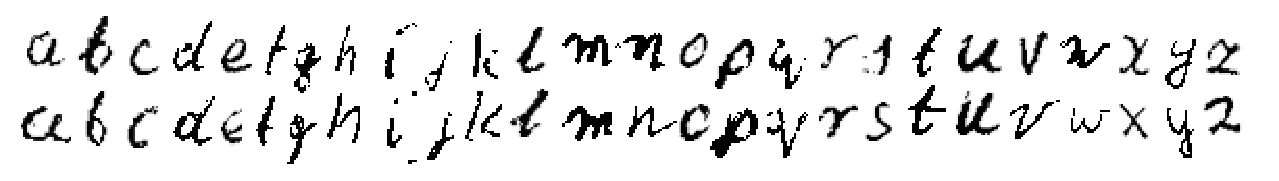
\includegraphics[width=0.7\textwidth]{_Figures/foreigns}
  \caption{Samples of native patterns -- handwritten digits and foreign patterns -- handwritten Latin alphabet letters.}
\label{fig:nativeforeignpatterns}
\end{figure}

All patterns were normalized and feature vectors comprising of 106 numerical features were created. Examples of features are: maximum/position of maximum values of projections, histograms of projections, transitions, offsets; raw moments, central moments, Euler numbers etc. We considered features standardization but the training data is sufficiently consistent (there are no outliers and the data is balanced), so we normalized those features to bring linearly all values into the range $[0,1]$. Best first search for the optimal feature subset has been performed using the FSelector R package,~\cite{Romanski}. The best first search is a~greedy search-based feature selection method. It is a~so called wrapper method, what means that we build multiple classification models based on various subsets of features and evaluate feature subset quality by checking classification accuracy on test set. We applied a~10-class SVM as an evaluator in this process. Next, we performed analysis of variance what led to further reduction of the feture set. Finally, the ready-to-use feature vector contained 24 elements. 



%-------------------------------------------------------------------
%-------------------------------------------------------------------

\subsection{Experimental Settings}
\vspace{-3pt}

We have formed the described three rejection mechanisms based on popular classification methods: SVM, random forest, kNN and we compare results obtained with those methods with results obtained with regression models: logistic regression and polynomial regression. 

The experiment presented in this paper has been conducted in Python programming language, using scientific libraries~\cite{NumPy,Scikit} and their implementations for SVM, Random Forests, kNN, logistic and polynomial regression. Several tests have been performed in order to find best suited method parameters for all classifiers by using Grid Search~\cite{Scikit} algorithm. Final results were obtained for SVM model with the Radial Basis Function kernel, cost parameter was tuned to be eight and \textcolor{red}{delta=0.5 ?? $\gamma$}. When using Random Forests a~total of 100 trees were used. kNN method used five neighbours when classifying. 


%-------------------------------------------------------------------
%-------------------------------------------------------------------
\subsection{Model Quality}
	\label{subsec:rejection_quality}

Experimental results are summarized in Tables~\ref{tab:results_classification_standard} (classification quality) and Table~\ref{tab:results_classification_regression} (rejection quality). 

\textcolor{red}{czemu jest "-- " w komorce Method2-kNN Fine accuracy?}

\textcolor{red}{Prosze umiescic dane z Tab 2 i Tab3 na jednym wykresie slupkowym - pewnie bedzie lepiej wygladalo i zaoszczedzimy troche miesjca. Prosze jeszcze sie upewnic czy wartosci sa dobrze przepisane. Rysujemy tylko dane estowe.}

\textcolor{red}{Prosze uzupelnic Tabelki 4 i 5. Prosze "wkleic" dane z tych tabelek tez do jednego excela i sprobowac narysowac z nich wykres (na razie pierwsza wersje -- zobaczymy czy zostaniemy przy tabelkach czy przy wykresie/wykresach). Rysujemy tylko dane testowe. }


\begin{table}[!htbp]
	\vspace{-12pt}
	\centering
	\caption{Classification quality obtained with an ensemble of binary classifiers based on popular models like SVM, random forests (RF) and kNN for the test (hold-out) set of native patterns.}
	\vspace{-3pt}
	\setlength{\tabcolsep}{5pt}
	\renewcommand{\arraystretch}{1}
	\footnotesize
	{	
		\begin{tabular}{|r||c|c|c||c|c|c||c|c|c|}
			\hline
			& \multicolumn{3}{c||}{Method 1} & \multicolumn{3}{c||}{Method 2} & \multicolumn{3}{c|}{Method 3}\\
			\hline
			Classifier & $\;\;$SVM$\;\;$ & $\;\;$RF$\;\;$ & $\,$kNN$\;\;$ & $\,$SVM$\;\;$ & $\;\;$RF$\;\;$ & $\,$kNN$\;\;$ & $\,$SVM$\;\;$ & $\;\;$RF$\;\;$ & $\,$kNN  \\
			\hline
			Strict Native Sens. & $0.903$ & $0.883$ & $0.806$ & $0.030$ & $0.097$ & $0$ & $0.964$ & $0.949$ & $0.926$ \\			
			Strict Accuracy  & $0.141$ & $0.178$ & $0.082$ & $0.737$ & $0.781$ & $0.8977$ & $0.259$ & $0.233$ & $0.094$ \\
			Fine Accuracy       & $0.910$ & $0.893$ & $0.806$ & $0.970$ & $0.963$ & $-$ & $0.969$ & $0.955$ & $0.926$ \\
			Accuracy  & $0.150$ & $0.190$ & $0.103$ & $0.737$ & $0.781$ & $0.898$ & $0.262$ & $0.239$ & $0.102$ \\
			\hline
		\end{tabular}	
	}
	\vspace{-0pt}
	\label{tab:results_classification_standard}
\end{table}

\begin{table}[!htbp]
	\vspace{-0pt}
	\centering
	\caption{Evaluation of classification quality for a~classifying/rejecting model based on polynomial and logistic regression achieved on the test set. }
	\vspace{-6pt}
	\setlength{\tabcolsep}{5pt}
	\renewcommand{\arraystretch}{1}
	{\footnotesize
		\begin{tabular}{|r||c|c||c|c||c|c|}
			\hline
			& \multicolumn{2}{c||}{Method 1} & \multicolumn{2}{c||}{Method 2} & \multicolumn{2}{c|}{Method 3}\\
			\hline
			Regression type & $\;\;$Polynomial$\;\;$ & $\,$Logistic$\;\;$ & $\,$Polynomial$\;\;$ & $\,$Logistic$\;\;$ & $\,$Polynomial$\;\;$ & $\,$Logistic  \\
			\hline
			Strict Native Sens. & $0.601$ & $0.727$ & $0.494$ & $0.030$ & $0.811$ & $0.920$ \\			
			Strict Accuracy  & $0.064$ & $0.114$ & $0.719$ & $0.820$ & $0.853$ & $0.143$ \\
			Fine Accuracy       & $0.602$ & $0.738$ & $0.969$ & $0.882$ & $0.959$ & $0.925$ \\
			Accuracy  & $0.105$ & $0.141$ & $0.720$ & $0.821$ & $0.587$ & $0.151$ \\			
			\hline			
		\end{tabular}	
	}
	\vspace{-0pt}
	\label{tab:results_classification_regression}
\end{table}


\begin{table}[!b]
	\vspace{-12pt}
	\centering
	\caption{ Quality of foreign patterns rejection/native patterns acceptance using proposed three methods based on popular algorithms: SVM, random forest and kNN. Results concern test set of native patterns mixed with the set of foreign elements (handwritten Latin alphabet letters).}
	\vspace{-6pt}
	\setlength{\tabcolsep}{5pt}
	\renewcommand{\arraystretch}{1}
	\footnotesize
	{
		\begin{tabular}{|r||c|c|c||c|c|c||c|c|c|}
			\hline
			& \multicolumn{3}{c||}{Method 1} & \multicolumn{3}{c||}{Method 2} & \multicolumn{3}{c|}{Method 3}\\
			\hline
			Classifier & $\;\;$SVM$\;\;$ & $\;\;$RF$\;\;$ & $\,$kNN$\;\;$ & $\,$SVM$\;\;$ & $\;\;$RF$\;\;$ & $\,$kNN$\;\;$ & $\,$SVM$\;\;$ & $\;\;$RF$\;\;$ & $\,$kNN  \\
			\hline
			Native Precision       & $0.107$ & $0.111$ & $0.102 $ & $0.057$ & $0.076$ & $-$ & $0.121$ & $0.118$ & $0.102$ \\
			Native Sensitivity & $0.993$ & $0.988$ & $1.000$ & $0.101$ & $0.102$ & $0.000$ & $0.995$ & $0.994$ & $1.000$ \\
			Native F--measure & $0.193$ & $0.200$ & $0.186$ & $0.073$ & $0.087$ & $-$ & $0.216$ & $0.211$ & $0.185$ \\
			Foreign Precision & $0.986$ & $0.987$ & $1.000$ & $0.888$ & $0.894$ & $0.898$ & $0.997$ & $0.996$ & $-$ \\
			Foreign Sensitivity & $0.054$ & $0.099$ & $0.000$ & $0.810$ & $0.859$ & $1.000$ & $0.179$ & $0.152$ & $0.000$ \\
			Foreign F--measure & $0.103$ & $0.179$ & $0.001$ & $0.847$ & $0.876$ & $0.946$ & $0.304$ & $0.264$ & $-$ \\			
			\hline
		\end{tabular}	
	}
	\vspace{-0pt}
	\label{tab:results_rejection_standard}
\end{table}


\begin{table}[!b]
	\vspace{-1pt}
	\centering
	\caption{Quality of foreign patterns rejection/native patterns acceptance for the three methods based on polynomial and logistic regression. Results concern test (hold-out set) of native patterns (handwritten digits) with the foreign set of handwritten letters.}
	\vspace{-6pt}
	\setlength{\tabcolsep}{3pt}
	\renewcommand{\arraystretch}{1}
	{\footnotesize
		\begin{tabular}{|r||c|c||c|c||c|c|}
			\hline
			& \multicolumn{2}{c||}{Method 1} & \multicolumn{2}{c||}{Method 2} & \multicolumn{2}{c|}{Method 3}\\
			\hline
			Regression type & $\;\;$Polynomial$\;\;$ & $\,$Logistic$\;\;$ & $\,$Polynomial$\;\;$ & $\,$Logistic$\;\;$ & $\,$Polynomial$\;\;$ & $\,$Logistic  \\
			\hline
			Native Precision       & &&&&& \\
			Native Sensitivity &&&&&&\\
			Native F--measure &&&&&&\\
			Foreign Precision &&&&&&\\
			Foreign Sensitivity &&&&&&\\
			Foreign F--measure &&&&&&\\			
			\hline			
		\end{tabular}	
	}
	\vspace{-0pt}
	\label{tab:results_rejection_regression}
\end{table}




\textcolor{blue}{Tu skonczylam czytac -- dokoncze sprawdzanie jak beda uzupelnione tabelki/wykresy, bo chce sie do nich odniesc w tekscie.}


As it can be seen, polynomial regression model achieved better accuracy in classifying native patterns and was better at rejecting the foreign ones than other tested models. It turned out that the third approach (Method 3) yielded the best results whereas the second one performed the worst. Method 2 was the one that ``destroyed'' classification capabilities of classifiers and had tendency to reject native patterns. On the other hand Method 1 accepted most of the foreign elements. Those results become more obvious if one looks at them from the methods' construction point of view. 

The first approach rejected input only after n failed tests which makes rejection less probable the more tests are performed (more native classes means more tests). Provided pattern was treated as native and labelled as an element from the first class that passed its corresponding test. Because tests were done in order (from class 1 to class n) we observed increased number of classified elements being treated as members from the first few classes.

The second method required certain class to be obviously ``stronger'' than the others in terms of classification. All patterns that had similarities between two or more different classes were rejected which resulted in poor classification capabilities. This result is not surprising given how often even people can be unsure what kind of handwritten symbol they see. Although it's not too hard for them to distinguish between a~letter and a~digit, correct classification of certain digits can be sometimes troublesome. Method~2 automatically rejected all symbols that were similar to two or more different classes. 

The third method provided some sort of equilibrium between classification and rejection by modifying method 2. Elements were rejected only when there was no strong evidence that they belong to certain class. This evidence was in fact the number of times pattern was assigned certain class' label. If there was no class with required number of labels the element was identified as a~foreign one. This approach can be compared to real-life situation where person classifies patterns by intuition and rejects them only when is really unsure about their true nature. 


%-------------------------------------------------------------------
%-------------------------------------------------------------------
%-------------------------------------------------------------------
\section{Conclusion}
  \label{sec:Conclusion}

Proposed solution for enhancing classifiers with rejection mechanism did not prove to yield good results for all models. Whereas SVM, Random Forests or kNN did not benefit from introduced changes, certain regression models indeed gained identification capabilities. It's worth noting that not every of the introduced methods performed well. In the conducted tests both method 1 and 2 were outperformed by method 3. This behaviour was analysed and explained in Section~\ref{subsec:rejection_quality}. 

We are aware that to truly confirm obtained results, test should be repeated on different data sets. Described in this paper set consisting of letters and digits, although being very large, might not match wide spectrum of problems. 

Let us conclude this paper by saying that various adaptations of the idea of enhancing classifiers with rejection capabilities has a~vital role in modern machine learning, especially when dealing with corrupted or unknown datasets. We believe that the study in this direction is worth further efforts.

%-------------------------------------------------------------------
%-------------------------------------------------------------------
%-------------------------------------------------------------------

\section*{Acknowledgement}

\noindent The research is partially supported  by the National Science Center, grant \\\mbox{No~2012/07/B/ST6/01501}, decision no \mbox{DEC-2012/07/B/ST6/01501}.

%-------------------------------------------------------------------
%-------------------------------------------------------------------
%-------------------------------------------------------------------
\begin{thebibliography}{1}
	

\bibitem{Altman1992}
Altman N. S., \emph{An introduction to kernel and nearest-neighbor nonparametric regression}. The American Statistician 46 (3), 1992, pp. 175-185.

\bibitem{Breiman2001}
Breiman, L., \emph{Random Forests}. Machine Learning 45 (1), 2001, pp. 5-32. 

\bibitem{BreunigKriegelNgSander1999}
Breunig, M. M., Kriegel, H. P., Ng, R. T., and Sander, J., \emph{OPTICS-OF: Identifying Local Outliers}, Proc. of European Conf. on Principles of Data Mining and Knowledge Discovery, 1999.

\bibitem{Chawla2006}
Chawla, S. and Sun, P., \emph{SLOM: a~new measure for local spatial outliers}, Knowl. Inf. Syst. 9(4), pp. 412--429, 2006.

\bibitem{CortesVapnik1995}
Cortes, C., Vapnik, V., \emph{Support-vector networks}. Machine Learning 20 (3), 1995, pp. 273-297.

\bibitem{Ghoting2008}
Ghoting, A., Parthasarathy, S. and Otey, M., \emph{Fast mining of distance-based outliers in high-dimensional datasets}, Data Min. Knowl. Discov. 16(3), pp. 349--364, 2008.

\bibitem{Grubbs1950}
Grubbs, F. E., \emph{Sample criteria for testing outlying observations}, Annals of Mathematical Statistics 21(1), pp. 27--58, 1950. 

\bibitem{He2003}
He, Z., Xu, X. and Deng, S., \emph{Discovering cluster-based local outliers}, Pattern Recognit. Lett. 24(9), pp. 1641--1650, 2003.

\bibitem{HempstalkFrankWitten2008}
Hempstalk, K., Frank, E. and Witten, I., \emph{One-class classification by combining density and class probability estimation}, Machine Learning and Knowl. Disc. in Databases, pp. 505--519, 2008.

\bibitem{Kapoor2010}
Kapoor, A., Grauman, K., Urtasun, R., and Darrell, T., \emph{Gaussian processes for object categorization}, Int. J. Comput. Vis. 88(2), pp. 169--188, 2010.

\bibitem{KimLee2006}
Kim, H. and Lee, J., \emph{Pseudo-density estimation for clustering with Gaussian processes}, Adv. Neural Netw. 3971, pp. 1238--1243, 2006.

\bibitem{KnorrNg1999}
Knorr, E. M. and Ng, R. T. \emph{Finding intensional knowledge of distance-based outliers}, Proc. of Int. Conf. on Very Large Data Bases, 1999.

\bibitem{LeCunCortesBurges}
LeCun, Y., Cortes, C., and Burges, C., \emph{The MNIST database of handwritten digits}, in: http://yann.lecun.com/exdb/mnist.

\bibitem{Paalanen2006}
Paalanen, P., Kamarainen, J., Ilonen, J. and Kalviainen, H., \emph{Feature representation
and discrimination based on Gaussian mixture model probability densities – practices and algorithms}, Pattern Recognition 39(7), pp. 1346--1358, 2006.

\bibitem{PimentelCliftonTarassenko2014}
Pimentel, M. A. F., Clifton, D. A., Clifton, L. and Tarassenko, L., \emph{A review of novelty detection}, Signal Processing 99, pp. 215--249, 2014.

\bibitem{Romanski}
Romanski, P., Kotthoff, L., \emph{Package FSelector}, http://cran.r-project.org/web/packages/FSelector/FSelector.pdf

\bibitem{NumPy}
http://www.numpy.org/

\bibitem{Scikit}
http://scikit-learn.org/stable/

\bibitem{Song2007}
Song, X., Wu, M., Jermaine, C., and Ranka, S., \emph{Conditional anomaly detection}, IEEE Trans. Knowl. Data Eng. 19(5), pp. 631--645, 2007.

\bibitem{Sun2004}
Sun, H., Bao, Y., Zhao, F., Yu, G. and Wang,D., \emph{CD-trees: an efficient index structure for outlier detection}, Adv. Web-Age Inf. Manage. 3129, pp. 600--609, 2004.

\bibitem{Tukey1977}
Tukey, J. W., \emph{Exploratory Data Analysis}, Addison-Wesley, 1977.
\end{thebibliography}

\end{document}


\begin{table}[!b]
	\vspace{-12pt}
	\centering
	\caption{ Results for classification with rejection when using popular models like SVM, Random Forests and kNN }
	\vspace{-6pt}
	\setlength{\tabcolsep}{3pt}
	\renewcommand{\arraystretch}{1}
	{\footnotesize
		\begin{tabular}{|r||c|c|c||c|c|c||c|c|c||c|c|c}
			\hline
			& \multicolumn{3}{c||}{Method 1} & \multicolumn{3}{c||}{Method 2} & \multicolumn{3}{c|}{Method 3}\\
			\hline
			Classifier & $\;\;$SVM$\;\;$ & $\;\;$RF$\;\;$ & $\,$kNN$\;\;$ & $\,$SVM$\;\;$ & $\;\;$RF$\;\;$ & $\,$kNN$\;\;$ & $\,$SVM$\;\;$ & $\;\;$RF$\;\;$ & $\,$kNN  \\
			\hline
			Data Set & \multicolumn{9}{c|}{Native Patterns, Train Set} \\
			\hline
			Accuracy &&&&&&&&&&&&\\
			Strict Accuracy     & $0.233$ & $0.269$ & $0.170$ & $0.660$ & $0.698$ & $0.790$ & $0.347$ & $0.330$ & $0.198$  \\
			%Fine Accuracy       & $0.912$ & $0.913$ & $0.813$ & $0.997$ & $1$ & $-$ & $0.984$ & $1$ & $0.949$ \\
			%Strict Native Sens. & $0.911$ & $0.913$ & $0.813$ & $0.095$ & $0.093$ & $0$ & $0.984$ & $1$ & $0.949$ \\
			Foreign Precision &&&&&&&&&&&&\\
			\hline
			Data Set & \multicolumn{9}{c|}{Native Patterns, Test Set} \\
			\hline
			Accuracy &&&&&&&&&&&&\\
			Strict Accuracy  & $0.141$ & $0.178$ & $0.082$ & $0.737$ & $0.781$ & $0.8977$ & $0.259$ & $0.233$ & $0.094$ \\
			%Fine Accuracy       & $0.910$ & $0.893$ & $0.806$ & $0.970$ & $0.963$ & $-$ & $0.969$ & $0.955$ & $0.926$ \\
			%Strict Native Sens. & $0.903$ & $0.883$ & $0.806$ & $0.030$ & $0.097$ & $0$ & $0.964$ & $0.949$ & $0.926$ \\
			Foreign Precision &&&&&&&&&&&&\\
			\hline
		\end{tabular}	
	}
	\vspace{-0pt}
	\label{tab:NativeNoForeign1}
\end{table}

\begin{table}[!b]
	\vspace{-0pt}
	\centering
	\caption{ Results for classification with rejection when using regression-based models }
	\vspace{-6pt}
	\setlength{\tabcolsep}{3pt}
	\renewcommand{\arraystretch}{1}
	{\footnotesize
		\begin{tabular}{|r||c|c||c|c||c|c||c|c|c|}
			\hline
			& \multicolumn{2}{c||}{Method 1} & \multicolumn{2}{c||}{Method 2} & \multicolumn{2}{c|}{Method 3}\\
			\hline
			Regression type & $\;\;$Polynomial$\;\;$ & $\,$Logistic$\;\;$ & $\,$Polynomial$\;\;$ & $\,$Logistic$\;\;$ & $\,$Polynomial$\;\;$ & $\,$Logistic  \\
			\hline
			Data Set & \multicolumn{6}{c|}{Native Patterns, Train Set} \\
			\hline
			Strict Accuracy     & $0.137$ & $0.186$ & $0.716$ & $0.726$ & $0.888$ & $0.236$ \\
			Fine Accuracy       & $0.645$     & $0.731$ & $1$ & $0.897$ & $1$ & $0.926$ \\
			Strict Native Sens. & $0.645$ & $0.720$ & $0.610$ & $0.030$ & $1$ & $0.921$ \\
			\hline
			Data Set & \multicolumn{6}{c|}{Native Patterns, Test Set} \\
			\hline
			Strict Accuracy  & $0.064$ & $0.114$ & $0.719$ & $0.820$ & $0.853$ & $0.143$ \\
			Fine Accuracy       & $0.602$ & $0.738$ & $0.969$ & $0.882$ & $0.959$ & $0.925$ \\
			Strict Native Sens. & $0.601$ & $0.727$ & $0.494$ & $0.030$ & $0.811$ & $0.920$ \\
			\hline
		\end{tabular}
	}
	\vspace{-6pt}
	\label{tab:NativeNoForeign2}
\end{table}

